%% =======================================================
%% 云南大学学位论文模板 (YNU-thesis)
%% =======================================================
%% Author: 赵苡积 (Dr. Zhao Yiji)
%% Institution: 云南大学 (Yunnan University)
%% Version: V1.0
%% =======================================================
%% 编译引擎: XeLaTeX (推荐)
%% =======================================================
%% type  选项: Bachelor (学士), Master (硕士), Doctor (博士)
%% print 选项: twoside (双面打印), oneside (单面打印)
%% =======================================================
\documentclass[type=Master, print=twoside]{style/YNU-thesis}

%% 指定图片路径
\graphicspath{{./figures/}}


%%%%%%%%%%%%%%%%% 填写封面信息 %%%%%%%%%%%%%%%%%%%%%%%%
% 硕博专属参数
\clc{}               % 分类号
\secretLevel{公开}    % 密级
\udc{}               % UDC
\serialNumber{}      % 编号


\title{YNUThesis：云南大学硕/博士学位论文\\ \LaTeX 模板——示例文档} %标题：长题目可用 \\ 手工分行
\englishtitle{YNUThesis: LaTeX Template for \\Yunnan University Master's and Doctoral \\Dissertations —— Sample Document}
\author{张三}
\studentNumber{2026100123}
\college{信息学院}
\major{计算机技术}
\researchArea{数据与知识工程}
\advisor{李四}
\advisorTitle{教授}
\datetime{2026 年 6 月}
%%%%%%%%%%%%%%%%%%%%%%%%%%%%%%%%%%%%%%%%%%%%%%%%%%%%


\begin{document}
	\makecover                             %封面
	\makereviewtable                       %简况表（本科无需填写）
	\begin{statement}

\branchByDegree{
    % =================================================
    % 本科生
    % =================================================
    本毕业论文（设计）是作者在导师指导下取得的成果。除了文中特别加以标注和致谢的地方外，论文（设计）中不包含其他人已经发表或撰写过的研究成果，不存在剽窃或抄袭行为。与作者一同工作的同志对本研究所做的任何贡献均已在论文中作了明确的说明并表示了谢意。

    现就论文（设计）的使用对云南大学授权如下：学校有权保留本论文（设计）（含电子版），也可以采用影印、缩印或其他复制手段保存论文（设计）；学校有权公布论文的全部或部分内容，可以将论文（设计）用于查阅或借阅服务；学校有权向有关机构送交学位论文（设计）用于学术规范审查、社会监督或评奖；学校有权将学位论文（设计）的全部或部分内容录入有关数据库用于检索服务。

    内部公开或保密的论文（设计）在解密后应遵循此规定。

    \vspace{44pt}

    \noindent{\heiti 作者签名：\underline{\makebox[7em][c]{}}\ \ \ \ 导师签名：\underline{\makebox[7em][c]{}}\ \ \ \ 日 \hskip 1em 期：\underline{\makebox[7em][c]{}}}
}{
    % =================================================
    % 硕/博研究生
    % =================================================
    本论文是作者在导师指导下取得的研究成果。除了文中特别加以标注和致谢的地方外，论文中不包含其他人已经发表或撰写过的研究成果，不存在剽窃或抄袭行为。与作者一同工作的同志对本研究所做的任何贡献均已在论文中作了明确的说明并表示了谢意。

    
    现就论文的使用对云南大学授权如下：学校有权保留本论文（含电子版），也可以采用影印、缩印或其他复制手段保存论文；学校有权公布论文的全部或部分内容，可以将论文用于查阅或借阅服务；学校有权向有关机构送交学位论文用于学术规范审查、社会监督或评奖；学校有权将学位论文的全部或部分内容录入有关数据库用于检索服务。
    
    {\heiti（内部公开或保密的论文（设计）在解密后应遵循此规定。）}

    \vspace{44pt}

    \noindent{研究生签名：\underline{\makebox[7em][c]{}}\ \ \ \ 导师签名：\underline{\makebox[7em][c]{}}\ \ \ \ 日 \hskip 1em 期：\underline{\makebox[7em][c]{}}}
}

\end{statement}


           %版权声明
	\frontmatter                           %摘要开始页脚用罗马体
	\begin{abstract}

摘要是毕业论文内容的高度概括，包括研究工作的目的和重要性、研究内容、方法和观点，以及研究取得的成果、结论和创新之处，应能反映论文的精华。摘要应具有独立性和完整性，不含图表和注释，无文献引用，语言力求精炼。

本科一般以300-500字为宜，硕士学位论文一般为500-1000字（一页以内），博士学位论文一般为1000-2000字。

关键词是反映毕业论文主题内容的核心词，是供检索使用的词条，应采用通用专业术语。关键词3-5个为宜，每个关键词的字数一般不超过5个；按词条外延层次（学科目录分类）由大至小顺序排列。各词之间用中文分号分隔，最末不用任何符号。 关键词要能体现论文的主要内容，词组符合学术规范；关键词应另起一行，排在摘要的下方，多个关键词之间用分号隔开。例如：

\keywords{摘要；硕士；博士}

\end{abstract}    %中文摘要
	\include{chapters/abstract_english}    %英文摘要
	\tableofcontents                       %目录

	%正文
	\mainmatter                     %正文开始页脚用阿拉伯数字
	\chapter{引言}
\label{cha:intro}

引言（或绪论）简要说明研究工作的目的、范围、相关领域的前人工作和知识空白、理论基础和分析、研究设想、研究方法和实验设计、预期结果和意义等。应言简意赅，不要与摘要雷同，不要成为摘要的注释。一般教科书中有的知识，在引言中不必赘述。

\section{背景}

学位论文为了需要反映出作者确已掌握了坚实的基础理论和系统的专门知识，具有开阔的科学视野，对研究方案作了充分论证，因此，有关历史回顾和前人工作的综合评述，以及理论分析等，可以单独成章，用足够的文字叙述。正文是学位论文的核心部分，占主要篇幅，可以包括：调查对象、实验和观测方法、仪器设备、材料原料、实验和观测结果、计算方法和编程原理、数据资料、经过加工整理的图表、形成的论点和导出的结论等。


由于研究工作涉及的学科、选题、研究方法、工作进程、结果表达方式等有很大的差异，对正文内容不能作统一的规定。但是，必须实事求是，客观真切，准确完备，合乎逻辑，层次分明，简练可读。

由于研究工作涉及的学科、选题、研究方法、工作进程、结果表达方式等有很大的差异，对正文内容不能作统一的规定。但是，必须实事求是，客观真切，准确完备，合乎逻辑，层次分明，简练可读。具体写作规范参考《云南大学本科毕业论文（设计）写作规范》\footnote{《云南大学本科毕业论文（设计）写作规范》：\url{https://co2.cnki.net/Notice.html?typeId=3596\&dp=ynu\&r=1776851073592}}，以及《云南大学研究生学位论文写作规范》\footnote{《云南大学研究生学位论文写作规范》：\url{http://www.grs.ynu.edu.cn/info/1036/1352.htm}}。




\section{二级标题}

命令：\textbackslash section\{二级标题\}。由于研究工作涉及的学科、选题、研究方法、工作进程、结果表达方式等有很大的差异，对正文内容不能作统一的规定。但是，必须实事求是，客观真切，准确完备，合乎逻辑，层次分明，简练可读。



\subsection{三级标题}

命令：\textbackslash section\{三级标题\}。实事求是，客观真切，准确完备，合乎逻辑，层次分明，简练可读。

\subsubsection{四级标题}

命令：\textbackslash subsubsection\{四级标题\}。必须实事求是，客观真切，准确完备，合乎逻辑，层次分明，简练可读。
    %第一章
	\chapter{常用的命令样例}
\label{cha:chap2}

写作规范参考《云南大学本科毕业论文（设计）写作规范》以及《云南大学研究生学位论文写作规范》。

\section{公式}

本模板定义了一些实用的命令，包括向量、矩阵、张量、引用公式命令。下面展示一些样例，便于论文撰写者使用：

\textbf{向量命令}：\textbackslash vec\{x\}：$\vec{x}$；
\textbf{矩阵命令}：\textbackslash mat\{x\}：$\mat{X}$；
\textbf{张量命令}：\textbackslash tensor\{x\}：$\tensor{X}$。

\textbf{公式引用命令}：引用公式时需要带有全角括号，可使用本模板定义的\textbackslash refeq\{\}命令，自带全角括号，例子：如公式\refeq{eq:ch2-split}所示。

\textbf{较长的上下标}，应使用非斜体\textbackslash mathrm\{xxx\}，如：$\vec{x}_{\mathrm{example}}^{\mathrm{example}}$。


\textbf{嵌入在文本中的行内公式}，使用\$\$命令，例子：$a + b = c$。

\textbf{单独为行的公式}，使用\textbackslash begin\{equation\}和\textbackslash end\{equation\}命令，较长的公式需要转行时，应尽可能在“$ = $”处回行，或者在“$ + $”、“$-$”“$*$”等记号处回行。例子：如公式\refeq{eq:ch2-split}、公式\refeq{eq:ch2-aligned}和公式\refeq{eq:ch2-align}所示。

\begin{equation}\label{eq:ch2-aligned}
	\begin{aligned}
		\dot{\hat{A}}^\dag
		&=\lambda_1\left(\tanh(k_3e_v)e_v-\sigma_1\hat{A}^\dag\right)\\
		&=\lambda_1\tanh(k_3e_v)e_v-\lambda_1\sigma_1\hat{A}^\dag
	\end{aligned}
\end{equation}


\begin{equation}\label{eq:ch2-split}
	\left\{
	\begin{aligned}
		\frac{\texttt{d}p(t)}{\texttt{d}t} &= v(t) \\
		\frac{\texttt{d}v(t)}{\texttt{d}t} &= u(t)-a(t)-b(t)v(t)-c(t)v^2(t)-f_2^*(\cdot)
	\end{aligned}
	\right.
\end{equation}




\begin{subequations}\label{eq:ch2-align}
	\begin{align}
		\dot{\hat{A}}^\dag&=\lambda_1\left(\tanh(k_3e_v)e_v-\sigma_1\hat{A}^\dag\right)\\
		\dot{\hat{b}}^\dag&=\lambda_2\left(|v||e_v|-\sigma_2\hat{b}^\dag\right)\\
		\dot{\hat{c}}^\dag&=\lambda_3\left(v^2|e_v|-\sigma_3\hat{c}^\dag\right)
	\end{align}
\end{subequations}



\section{定理}

\begin{Definition}
	这是一个定义。
\end{Definition}

\begin{Theorem}
	这是一个定理。
\end{Theorem}

\begin{Lemma}
	这是一个引理。
\end{Lemma}

\begin{Proof}
	这是一个证明。
	\qed
\end{Proof}


\section{代码}

代码示例：

\begin{lstlisting}[language=Python]
# ================= 冒泡排序算法实现 =================
def bubble_sort(arr):
    n = len(arr)
    # 遍历所有数组元素
    for i in range(n):
        # Last i elements are already in place
        for j in range(0, n-i-1):
            # 如果当前元素大于下一个元素，则交换它们
            if arr[j] > arr[j+1]:
                arr[j], arr[j+1] = arr[j+1], arr[j]
    return arr

# 测试代码
if __name__ == "__main__":
    my_list = [64, 34, 25, 12, 22, 11, 90]
    sorted_list = bubble_sort(my_list)
    print("排序后的数组:", sorted_list)
\end{lstlisting}

\section{算法}
本模板基于algorithm2e包制作了简单的中文算法表格，如算法\ref{algo:ch2-demo}所示。

\begin{centeralgo}[htbp]{0.65\textwidth}
    \onehalfspacing 
    \LinesNumbered
    \caption{图卷积前向传播算法}
    \label{algo:ch2-demo}
    \KwIn{张量$\tensor{X}$，矩阵$\mat{A}$，层数$L$}
    \KwOut{特征$\mat{H}$}

    \tcp{训练模型}
    \While{不满足早停条件}{
        初始化隐状态 $\mat{H}^{(0)} = \tensor{X}$\;
        \For{$l = 0$ \KwTo $L-1$}{
            \tcp{计算图卷积聚合}
            $\mat{H}^{(l+1)} = \sigma \left( \tilde{\mat{A}} \mat{H}^{(l)} \mat{W}^{(l)} + \vec{b}^{(l)} \right)$\;
        }
    }
    \Return $\mat{H}^{(L)}$
\end{centeralgo}


%
\section{图片}

插图之前，文中必须有关于本插图的提示，如“见图\ref{fig:ch2-f1}”、“如图\ref{fig:ch2-f1}所示”等。非特殊情况，图中文字应为中文，同一幅图内文字格式应统一，物理量、符号用斜体。\textbf{单图}，如图\ref{fig:ch2-f1}所示。\textbf{多图并列}，如图\ref{fig:ch2-f2}所示。


\begin{figure}[!htb]
	\centering
	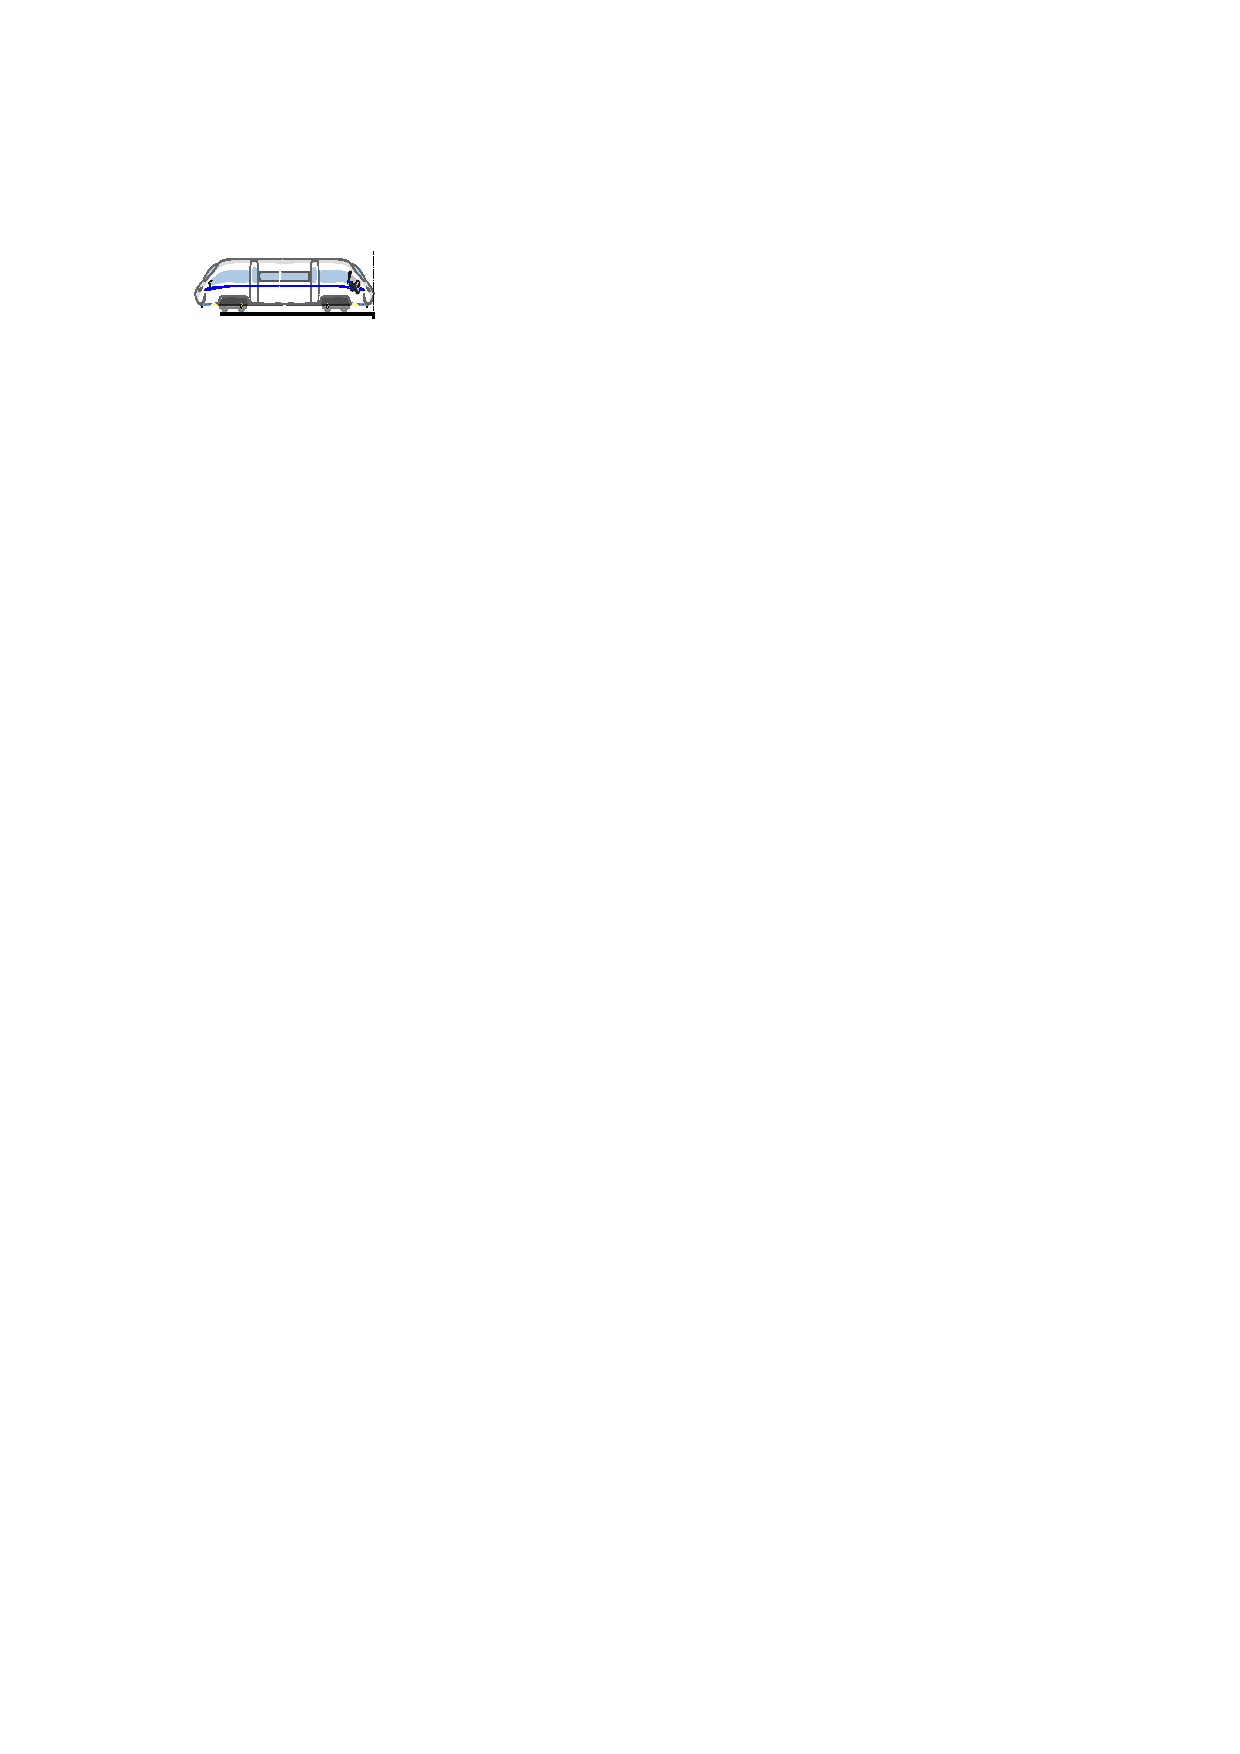
\includegraphics[scale=0.95]{figures/ch2/figure1.pdf}
	\caption{单图示意图}
	\label{fig:ch2-f1}
\end{figure}




\begin{figure}[!htb]
	\centering
	% 第一个子图环境，0.45\textwidth 控制子图占用的宽度比例
	\begin{subfigure}[b]{0.45\textwidth}
		\centering
		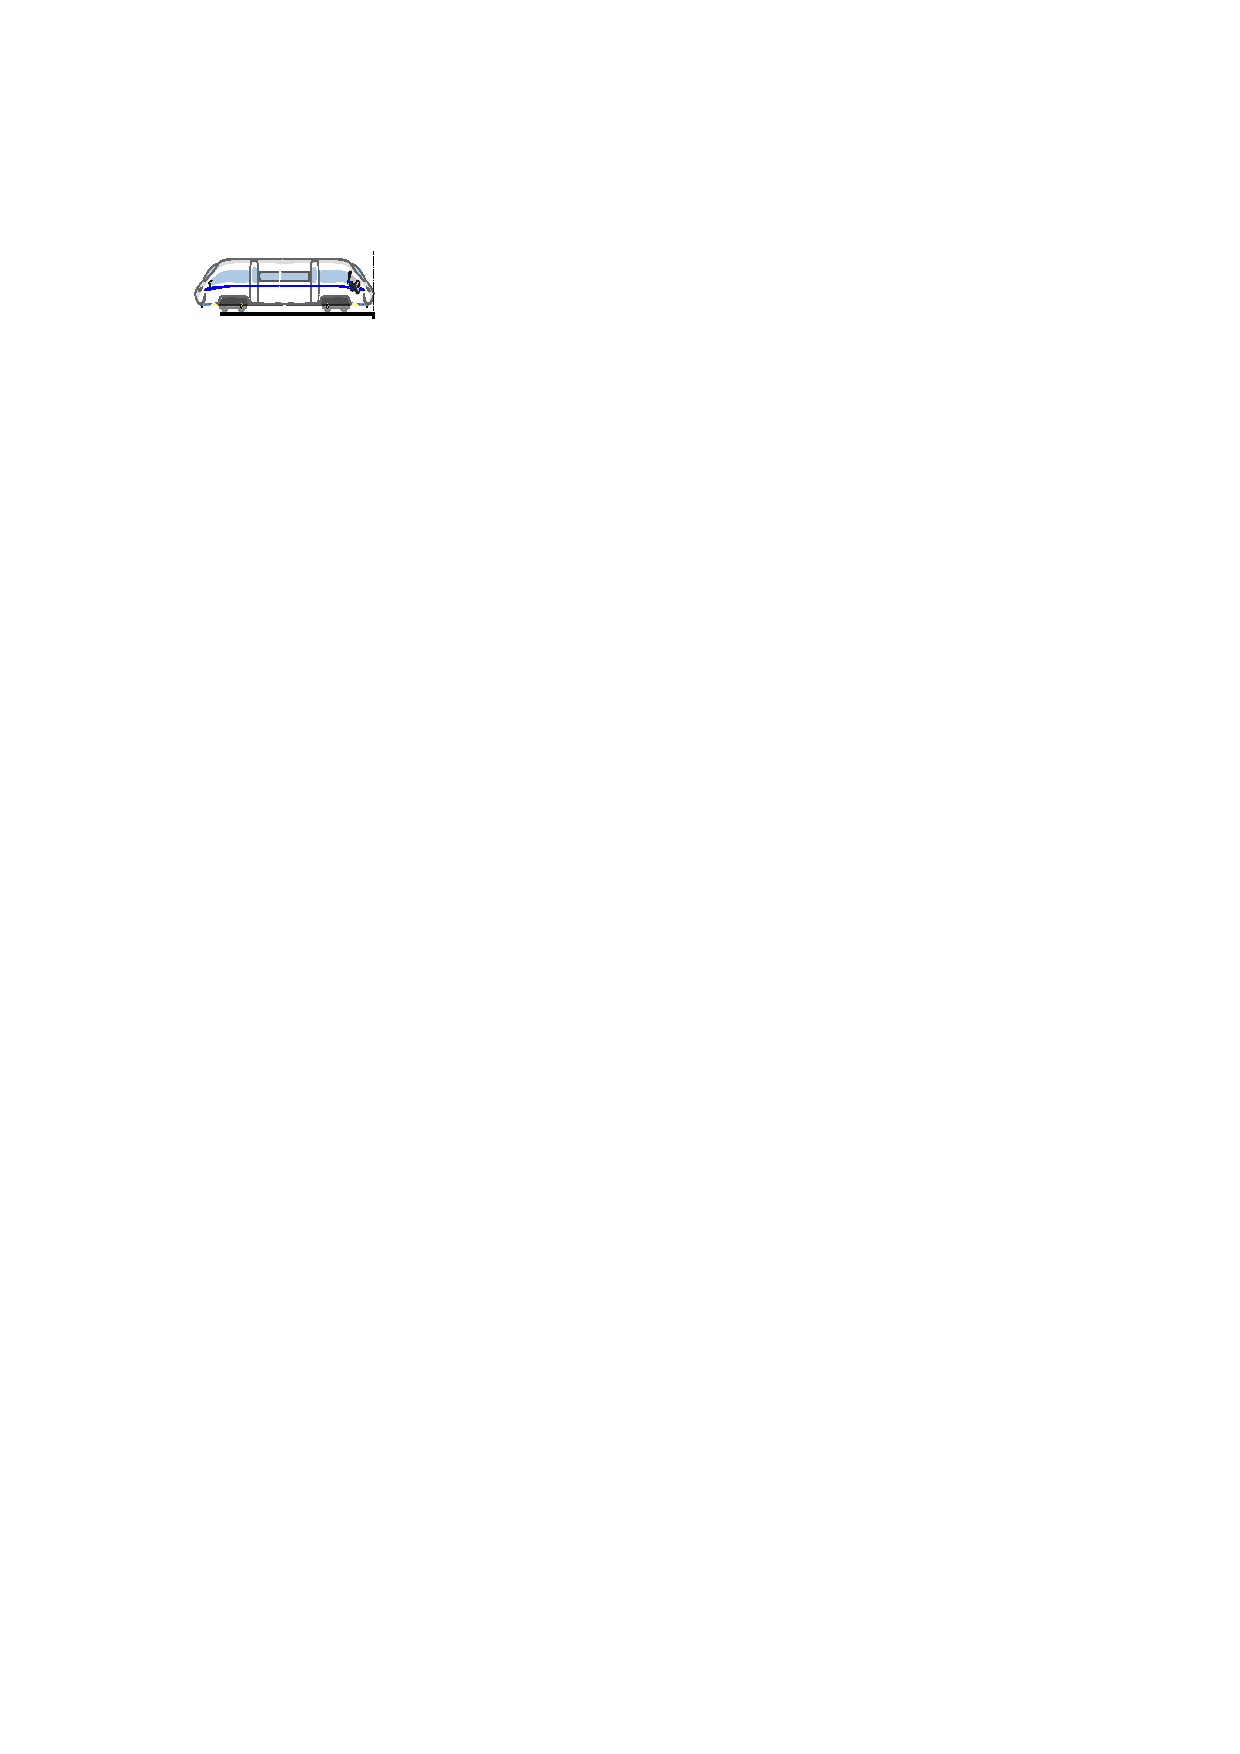
\includegraphics[scale=1]{figures/ch2/figure1.pdf}
		% 在 subcaption 中，直接用 \\ 换行就可以实现双语标题，不需要改计数器！
		\caption{子图1} 
		\label{fig:ch2-sub1}
	\end{subfigure}
	\hspace{5pt} % 子图间距，也可以用 \hfill 让它们自动靠两边对齐
	% 第二个子图环境
	\begin{subfigure}[b]{0.45\textwidth}
		\centering
		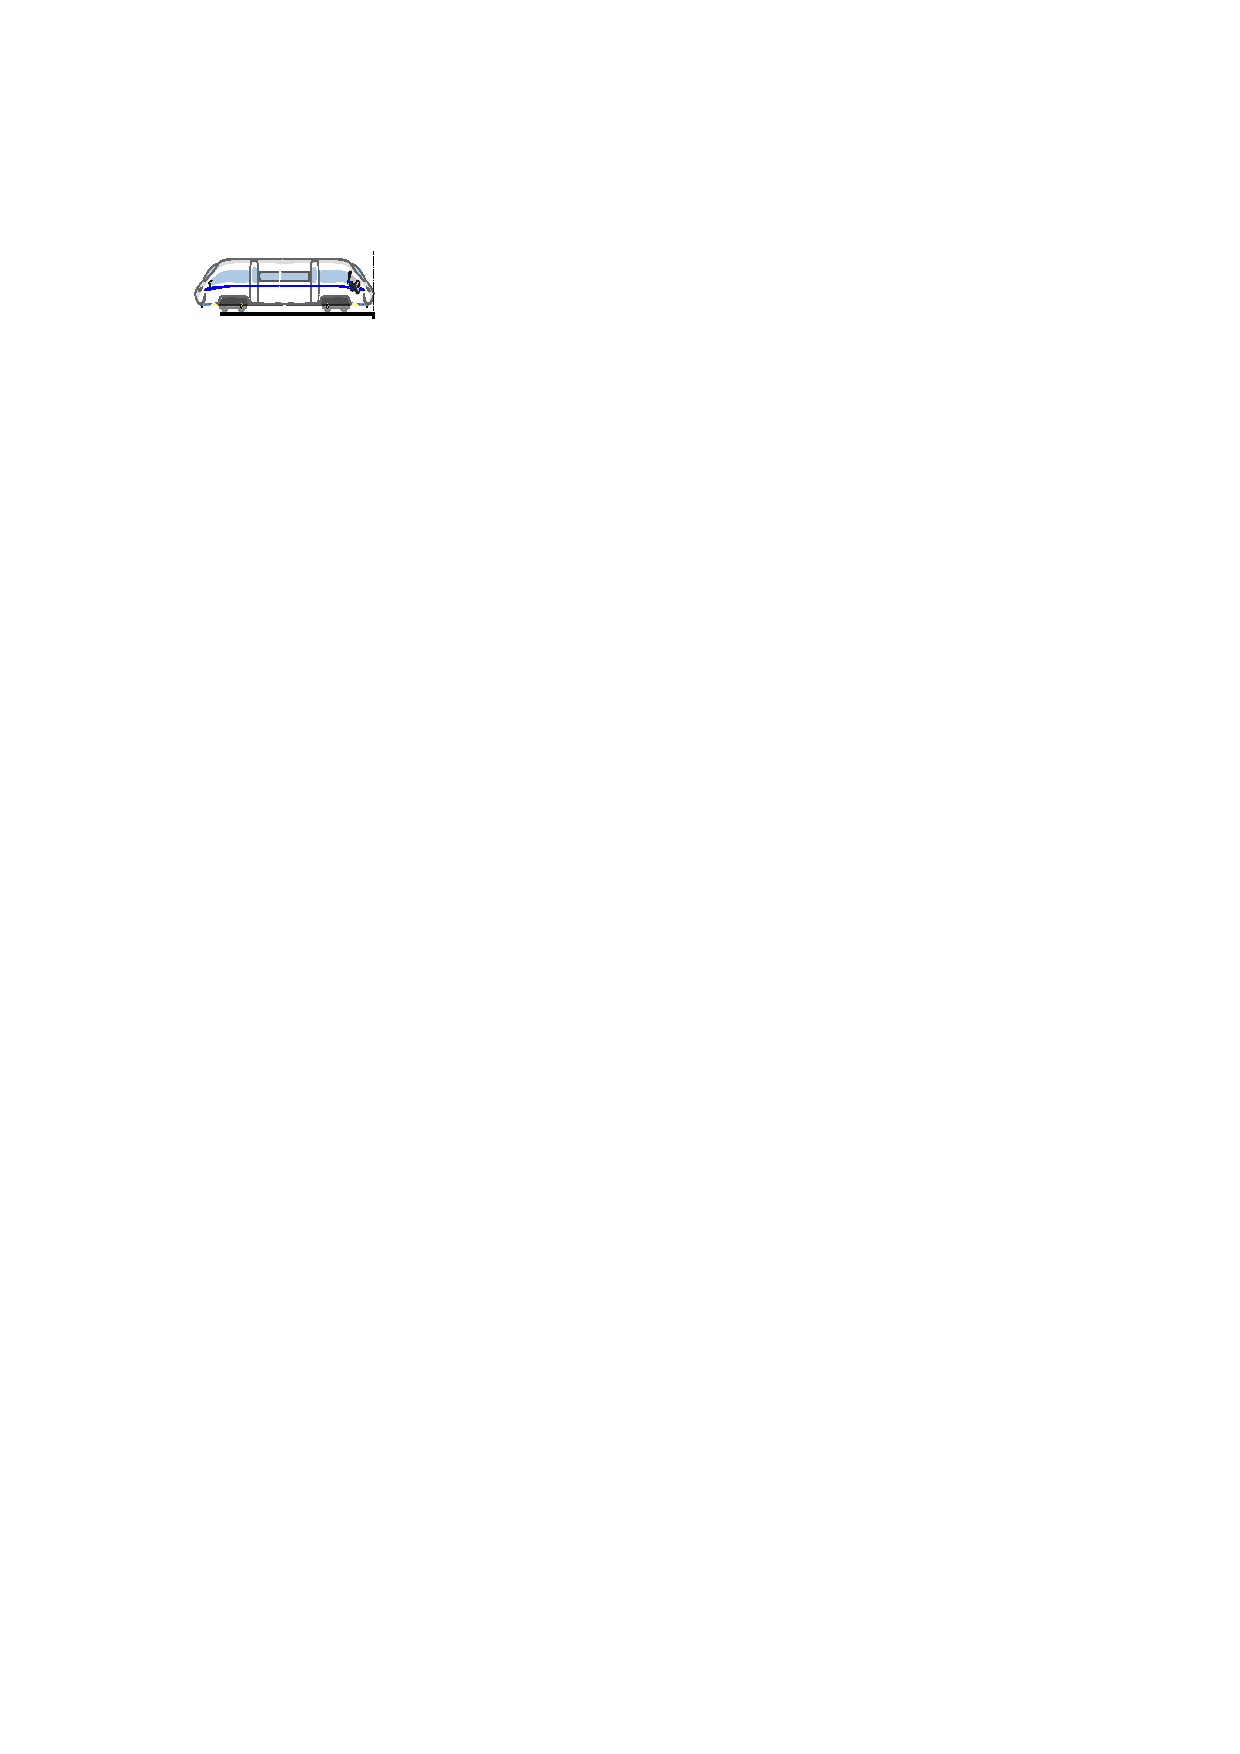
\includegraphics[scale=1]{figures/ch2/figure1.pdf}
		\caption{子图2}
		\label{fig:ch2-sub2}
	\end{subfigure}

        % 第三个子图环境
	\begin{subfigure}[b]{0.45\textwidth}
		\centering
		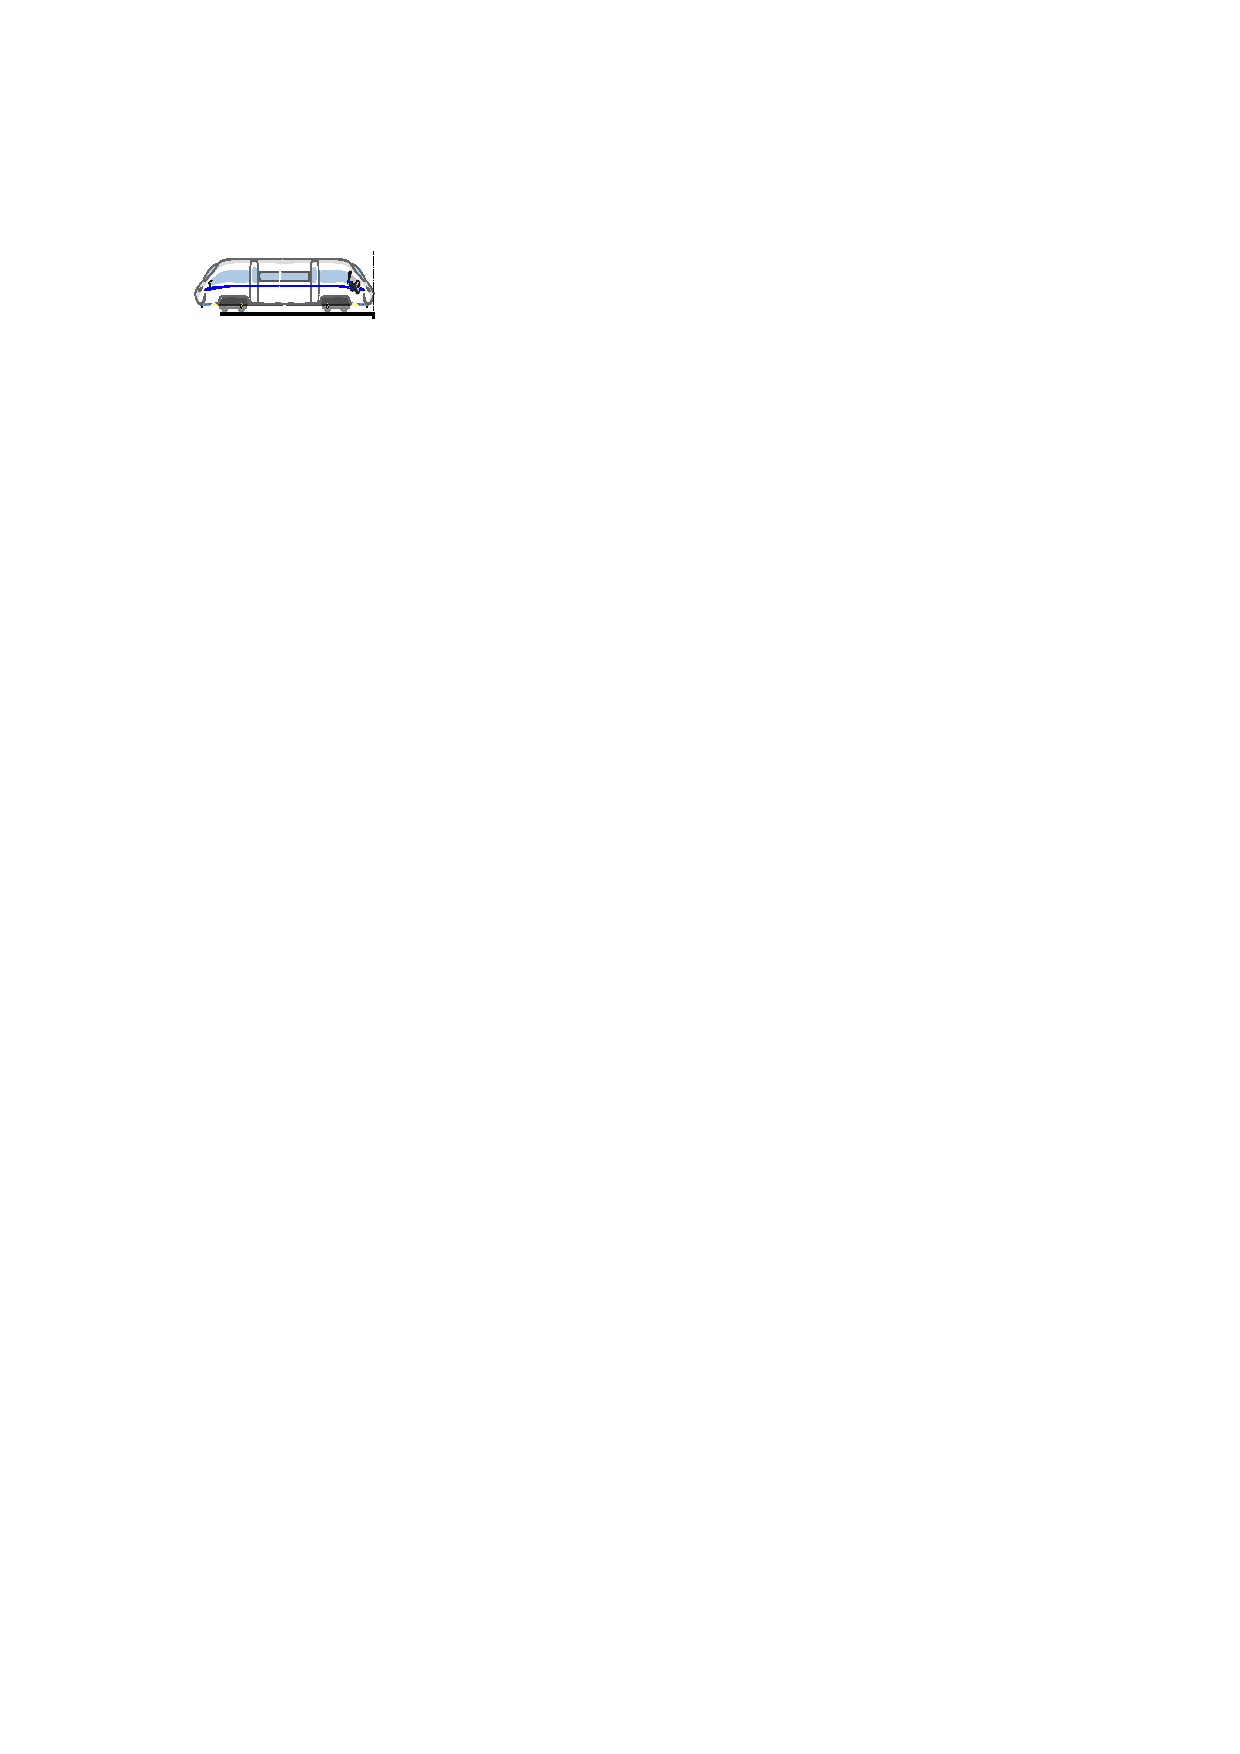
\includegraphics[scale=1]{figures/ch2/figure1.pdf}
		% 在 subcaption 中，直接用 \\ 换行就可以实现双语标题，不需要改计数器！
		\caption{子图3} 
		\label{fig:ch2-sub3}
	\end{subfigure}
	\hspace{5pt} % 子图间距，也可以用 \hfill 让它们自动靠两边对齐
	% 第四个子图环境
	\begin{subfigure}[b]{0.45\textwidth}
		\centering
		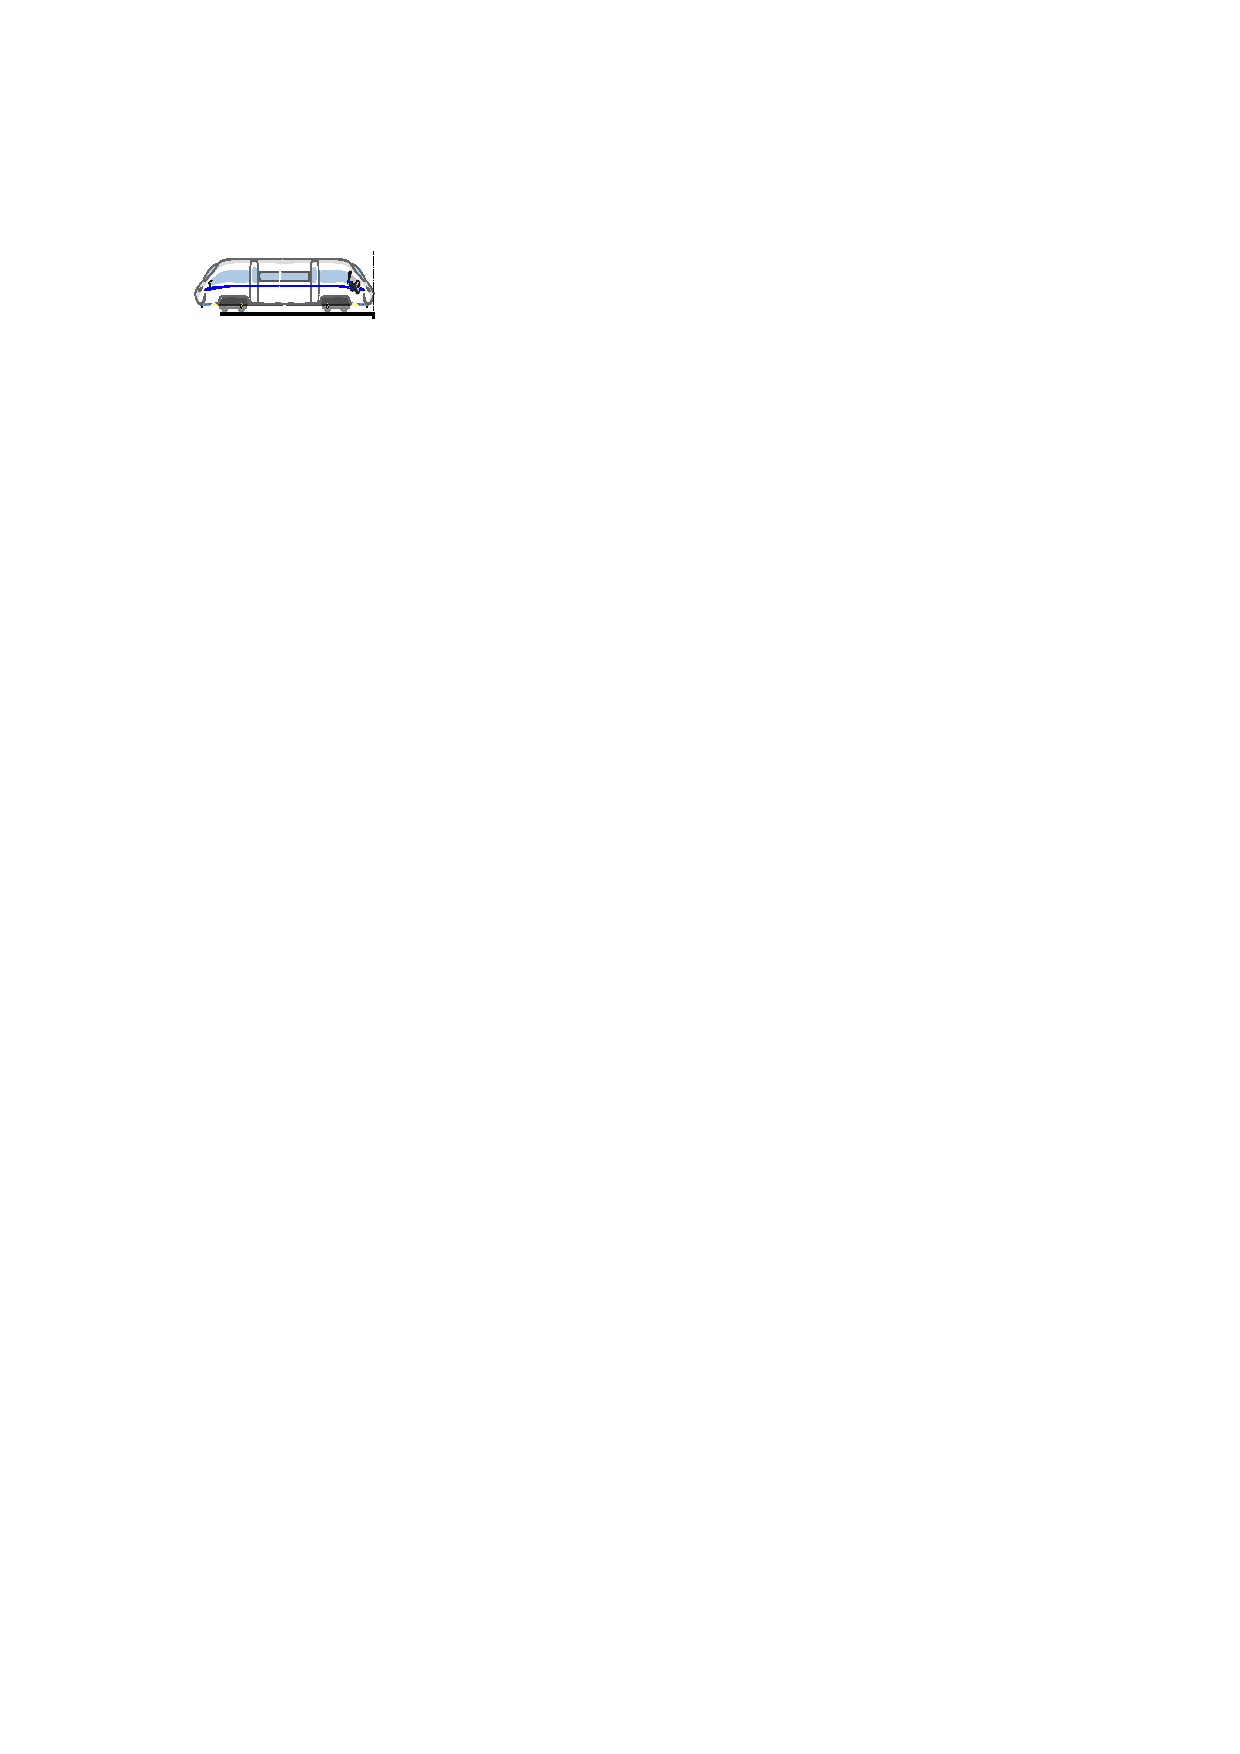
\includegraphics[scale=1]{figures/ch2/figure1.pdf}
		\caption{子图4}
		\label{fig:ch2-sub4}
	\end{subfigure}
	\caption{多图并列示意图}
	\label{fig:ch2-f2}
\end{figure}




\section{表格}

表题置于表的上方，居中。表格的编排建议采用国际通行的三线表，不加左、右边框线。表中文字用宋体（中文）或Times New Roman字体（英文）。

\textbf{带脚注的三线表}：如表\ref{tab:ch2_res1}所示，标题中写不下的内容可放至脚注，此时使用threeparttable包来实现。如果表格超出页面边距或内容太过拥挤，可以使用\textbackslash tabcolsep命令来调节列间距。

\textbf{巨型表格}：表格过大且无法拆分成多个表格时，可以使用sidewaystable旋转表格独占一页，本模板已添加旋转包，只需将\textbackslash begin\{table\}和\textbackslash end\{table\}命令中的table换为sidewaystable即可。如表\ref{tab:ch2_res3}所示。


\begin{table}[!htb]
	\centering
	\small %字体大小
	%\setlength\tabcolsep{3.3pt} %调整列间距
	\caption{性能对比。}
	\begin{threeparttable}
		\begin{tabular}{c|ccc|ccc}
			\toprule
			\multirow{2}{*}{模型} &  & 数据集1 &  &  & 数据集2&  \\
			& MAE & RMSE & MAPE(\%) & MAE & RMSE & MAPE(\%) \\
			\midrule
			
			SVR & 46.46 & 92.97 & 83.40 & 11.10 & 19.84 & 91.96  \\
			LSTM & \textbf{36.20 $\pm$0.17} & \textbf{66.26 $\pm$0.80} & \textbf{40.42 $\pm$0.86} & \textbf{6.70 $\pm$0.02} & \textbf{11.36 $\pm$0.04} & \textbf{74.01 $\pm$1.26}  \\
			\bottomrule
		\end{tabular}
		\begin{tablenotes}
			\footnotesize
			\item[*] 粗体代表所有基准模型中的最佳的性能。
		\end{tablenotes}
	\end{threeparttable}
	\label{tab:ch2_res1}
\end{table}



% 独占一页的表格样例
\begin{sidewaystable}[!htp]
	%\small %字体大小
	\setlength\tabcolsep{20pt} %调整列间距
	\caption{性能对比}
	\begin{threeparttable}
		\begin{tabular}{c|ccc|ccc}
			\toprule
			\multirow{2}{*}{模型} &  & 数据集1 &  &  & 数据集2&  \\
			& MAE & RMSE & MAPE(\%) & MAE & RMSE & MAPE(\%) \\
			\midrule
			
			SVR & 46.46 & 92.97 & 83.40 & 11.10 & 19.84 & 91.96  \\
			LSTM & 36.20 $\pm$0.17 & 66.26 $\pm$0.80 & 40.42 $\pm$0.86 & 6.70 $\pm$0.02 & 11.36 $\pm$0.04 & 74.01 $\pm$1.26  \\
			LSTM & 36.20 $\pm$0.17 & 66.26 $\pm$0.80 & 40.42 $\pm$0.86 & 6.70 $\pm$0.02 & 11.36 $\pm$0.04 & 74.01 $\pm$1.26  \\
			LSTM & 36.20 $\pm$0.17 & 66.26 $\pm$0.80 & 40.42 $\pm$0.86 & 6.70 $\pm$0.02 & 11.36 $\pm$0.04 & 74.01 $\pm$1.26  \\
			LSTM & 36.20 $\pm$0.17 & 66.26 $\pm$0.80 & 40.42 $\pm$0.86 & 6.70 $\pm$0.02 & 11.36 $\pm$0.04 & 74.01 $\pm$1.26  \\
			LSTM & 36.20 $\pm$0.17 & 66.26 $\pm$0.80 & 40.42 $\pm$0.86 & 6.70 $\pm$0.02 & 11.36 $\pm$0.04 & 74.01 $\pm$1.26  \\
			LSTM & 36.20 $\pm$0.17 & 66.26 $\pm$0.80 & 40.42 $\pm$0.86 & 6.70 $\pm$0.02 & 11.36 $\pm$0.04 & 74.01 $\pm$1.26  \\
			LSTM & 36.20 $\pm$0.17 & 66.26 $\pm$0.80 & 40.42 $\pm$0.86 & 6.70 $\pm$0.02 & 11.36 $\pm$0.04 & 74.01 $\pm$1.26  \\
			LSTM & 36.20 $\pm$0.17 & 66.26 $\pm$0.80 & 40.42 $\pm$0.86 & 6.70 $\pm$0.02 & 11.36 $\pm$0.04 & 74.01 $\pm$1.26  \\
			LSTM & 36.20 $\pm$0.17 & 66.26 $\pm$0.80 & 40.42 $\pm$0.86 & 6.70 $\pm$0.02 & 11.36 $\pm$0.04 & 74.01 $\pm$1.26  \\
			LSTM & 36.20 $\pm$0.17 & 66.26 $\pm$0.80 & 40.42 $\pm$0.86 & 6.70 $\pm$0.02 & 11.36 $\pm$0.04 & 74.01 $\pm$1.26  \\
			LSTM & 36.20 $\pm$0.17 & 66.26 $\pm$0.80 & 40.42 $\pm$0.86 & 6.70 $\pm$0.02 & 11.36 $\pm$0.04 & 74.01 $\pm$1.26  \\		
			LSTM & 36.20 $\pm$0.17 & 66.26 $\pm$0.80 & 40.42 $\pm$0.86 & 6.70 $\pm$0.02 & 11.36 $\pm$0.04 & 74.01 $\pm$1.26  \\
			LSTM & 36.20 $\pm$0.17 & 66.26 $\pm$0.80 & 40.42 $\pm$0.86 & 6.70 $\pm$0.02 & 11.36 $\pm$0.04 & 74.01 $\pm$1.26  \\
			LSTM & 36.20 $\pm$0.17 & 66.26 $\pm$0.80 & 40.42 $\pm$0.86 & 6.70 $\pm$0.02 & 11.36 $\pm$0.04 & 74.01 $\pm$1.26  \\
			LSTM & 36.20 $\pm$0.17 & 66.26 $\pm$0.80 & 40.42 $\pm$0.86 & 6.70 $\pm$0.02 & 11.36 $\pm$0.04 & 74.01 $\pm$1.26  \\
			LSTM & \textbf{36.20 $\pm$0.17} & \textbf{66.26 $\pm$0.80} & \textbf{40.42 $\pm$0.86} & \textbf{6.70 $\pm$0.02} & \textbf{11.36 $\pm$0.04} & \textbf{74.01 $\pm$1.26}  \\
			\bottomrule
		\end{tabular}
		\begin{tablenotes}
			\footnotesize
			\item[*] 粗体代表所有基准模型中的最佳的性能。
		\end{tablenotes}
	\end{threeparttable}
	\label{tab:ch2_res3}
\end{sidewaystable}


    %第二章
	\chapter{参考文献格式说明}
\label{cha:chap3}


\section{参考文献格式说明}

\textbf{命令：}\textbackslash cite\{xxx\}，如深度学习\cite{lecunDeepLearning2015}，中文文献\cite{zhou2021}。


\textbf{参考文献检查项}：论文完成后应仔细检查参考文献格式，下面总结了一些在论文审阅过程中常被指出的问题：

\begin{itemize}
	\item 参考文献格式参照节\ref{subsec:ref}
	\item 除Arxiv文章，所有文献必须有页码、年份，期刊论文还应有卷号、期号
	\item 检查同一会议/期刊的名称是否统一
	\item 检查文献标题单词首字母大写是否统一
	\item 检查是否有重复文献
\end{itemize}








\subsection{参考文献格式}\label{subsec:ref}

参考文献是文中引用的有具体文字来源的文献集合。按照GB 7714《文后参考文献著录规则》的规定执行。参考文献的格式为:

著作：[序号]作者.译者.书名[M].版本(第一版不著录).出版地:出版社,出版时间:引用部分起止页.

期刊：[序号]作者.译者.文章题目[J].期刊名,年份,卷号(期数):引用部分起止页.

会议论文集：[序号]作者.译者.文章名[C]. //编者.论文集名,会议地址，会议时间.出版地:出版者，出版年.引用部分起止页.

学位论文：[序号]作者.题名[D].保存地点:保存单位,年份.引用部分起止页.

专利：[序号]专利申请者.专利文献题名[P].国别,专利文献种类,专利号.发布日期:引用部分起止页.

技术标准：[序号]起草责任者.标准代号.标准顺序号——发布年.标准名称.出版地.出版者.出版年份:引用部分起止页.

报纸: [序号]作者.题名[N].报纸名，出版日期(版次)


    %第三章
	\include{chapters/chapter04}    %第四章
	\include{chapters/chapter05}    %第五章
	\include{chapters/chapter_conclusion}    %总结与展望


	%参考文献
	\bibliography{ref}
	\begin{mresume}

%%% 作者简历及成果，本科无需填写

\section*{一、作者简历}

xxxxxxxx。



\section*{二、发表论文}

\begin{enumerate}[leftmargin=*, parsep=5pt, label={[\arabic*]}]

	%非匿名
	\item \textbf{Author1}, Author2. Title. \emph{Journal/Conference}, Year, Volume(Issue), Pages. (CCF 类别，SCI分区)
	
	%匿名
	\item \textbf{第一作者}. Title. \emph{Journal/Conference}, Year, Volume(Issue), Pages. (CCF 类别，SCI分区)
	
\end{enumerate}




\section*{三、参与科研项目}

\begin{enumerate}[leftmargin=*, parsep=5pt, label={[\arabic*]}]
	
	\item xxxxxx。
	
	\item xxxxxx。

\end{enumerate}



\section*{四、获奖情况}

\begin{enumerate}[leftmargin=*, parsep=5pt, label={[\arabic*]}]
	
	\item xxxxxx。
	
	\item xxxxxx。
	
\end{enumerate}


\end{mresume}      %作者简历（本科无需填写）
	\begin{thanks}
	
对导师和给予指导或协助完成毕业论文的组织和个人表示感谢。致谢文字要简洁、实事求是，切忌浮夸，不得照搬照抄。


\end{thanks}       %致谢


\end{document}




















